\chapter{Technische Grundlagen}
\label{ch:background}
In diesem Kapitel werden alle nötigen technischen Grundlagen zusammengetragen. Da es sich um ein OAuth2 System handelt, wird diese Spezifikation erläutert. Zudem werden auf die Tokens eingegangen, die die Ressource Server jeweils validieren müssen. Diese sind \ac{JSON} Web Token. Dann werden noch die Metriken zum Messen der Performance erläutert, das Programm zum Messen dieser Werte genannt sowie das Framework zur Implementierung der Ressource Server erklärt. 

%
% Section: Der erste Abschnitt
%
\section{Grundlegender Begriffe der IT-Sicherheit}
\label{sec:background:first_section}
Im Bereich der IT-Sicherheit gibt es eine Reihe relevanter Begriffe, die regelmäßig verwendet werden.

\begin{description}
  \item[Authentifizierung:] Bei einer Authentifizierung beweist ein Nutzer seine Identität, indem er dem gegenüberliegenden Server Informationen übermittelt, über die nur der Nutzer verfügen kann wie beispielsweise ein Nutzername und Passwort oder ein Token.
  \item[Autorisierung:] Eine Autorisierung findet grundsätzlich nach der Authentifizierung statt. Hier überprüft das System nach der Authentifizierung des Nutzers, ob der Nutzer über die notwendigen Rechte verfügt eine Aktion auszuführen. 
  \item[Integrität:] Bei der Integrität wird verifiziert, dass Daten seit ihrer Erstellung nicht verändert wurden. Dies kann beispielsweise durch eine Signatur, die nur der Ersteller der Daten erstellen kann, gewährleistet werden [5].
  \item[Authentizität:] Das Ziel der Authentizität ist die Verifizierung des Erstellers der Daten [5]. Das bedeutet, es soll möglich sein zu überprüfen, dass die Daten, die zugesendet werden, auch tatsächlich von der Person oder dem System kommen, von der man annimmt das sie der Urheber ist.
  \item[Validierung] Man kann von einer Validierung sprechen, wenn oben genannte Aspekte, nämlich die Authentifizierung, Autorisierung, Integrität sowie Authentizität, überprüft werden.
\end{description}

%
% Section: Der Zweite Abschnitt
%
\section{OAuth2}
\label{sec:background:second_section}
OAuth2 ist eine Spezifikation, die ursprünglich entwickelt wurde, um Dritten Zugriff auf die Daten eines sogenannten Ressource Owners zu ermöglichen, ohne dass dieser Ressource Owner dem Dritten, in der Spezifikation Client genannt, sein Nutzername und Passwort übermitteln muss [6].  Dies wird dadurch ermöglicht, dass dem Client von einem Autorisationsserver ein Token übermittelt wird und mit diesem Token kann der Client Daten des Ressource Owners abfragen oder Aktionen im Namen des Ressource Owners durchführen. Diese Daten des Ressource Owners werden auf dem sogenannten Ressource Server gehostet.
Im Laufe der Zeit wurde diese Spezifikation erweitert, um weitere Anwendungsfälle abzudecken, wie die Spezifikation OpenID Connect, welche Single-Sign-On ermöglicht. 

\subsection{Rollen in OAuth2}
\label{subsec:background:second_section:first_subsection}
Es gibt vier verschiedene Rollen, die in OAuth2 spezifiziert sind.

\begin{description}
  \item[Ressource Owner:] Der Ressource Owner ist dazu in der Lage, Dritten Zugriff auf seine Daten zu geben oder Aktionen in seinem Namen durchzuführen [7]. Falls der Ressource Owner eine Person ist, nennt man ihn den End-Nutzer.
  \item[Ressource Server:] Der Ressource Server hostet die geschützten Ressourcen des Ressource Owners und ist in der Lage Anfragen zu diesen Ressourcen zu beantworten, falls ein valider Token, ein sogenannter Access Token, in der Anfrage zur Ressource vorliegt [7].
  \item[Client:] Der Client ist diejenige Komponente, die die Ressource des Ressource Owner's von dem Ressource Servers erlangen möchte und dafür einen Access Token benötigt [7]. 
  \item[Authorization Server:] Der Authorization Server verteilt Access Token falls sich der Ressource Owner erfolgreich authentifiziert und gegebenenfalls den Client autorisiert hat, Aktionen durchzuführen. 
\end{description}

\subsection{Erhalt von Token}
\label{subsec:background:second_section:second_subsection}

Gemäß der Spezifikation gibt es fünf verschiedene Wege, wie ein Client von einem Authorization Server einen Token erhalten kann [8]. Im Folgenden werden nur lediglich zwei beschrieben, da die anderen drei für diese Arbeit keine Relevanz haben. 

\subsubsection{Authorization Code Grant}
\label{ssubsec:background:second_section:first_subsection:first_subsubsection}
Bei dem Authorization Code Grant wird der Ressource Owner, der einen Webbrowser verwendet, von dem Client auf den Authorization Server weitergeleitet, um den Ressource Owner zu bitten, sich bei dem Authorization Server zu authentifizieren, um dann dem Client zu autorisieren auf eine geschützte Ressource des Ressource Servers zuzugreifen [9]. 

\begin{figure}[htbp]
  \centering
  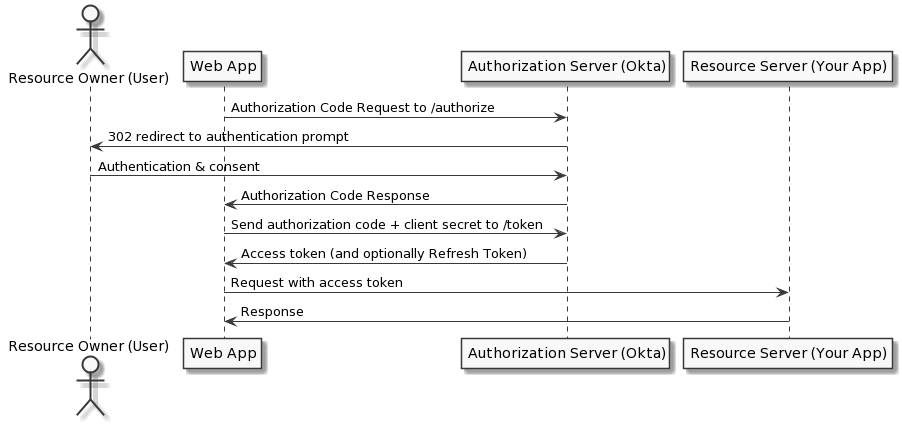
\includegraphics[width=1.0\textwidth]{gfx/oauth_auth_code_flow.png}
  \caption{Authorization Code Grant}
  \label{fig:chapter02:oauth_auth_code_flow}
 \end{figure}

In Abbildung 2.1 ist der Authorization Code Grant Flow als Sequenzdiagramm abgebildet. Es ist offensichtlich, dass es Beziehungen zwischen allen vier Rollen gibt, nämlich dem Ressource Owner, dem Client, in diesem Fall als „Web App“ gekennzeichnet, dem Authorization Server, Okta, und dem Ressource Server. 
Grob kann man es sich in der Praxis so vorstellen, dass ein Nutzer eine Webapplikation (=Client) bedient und diese Webapplikation möchte, dass der Nutzer sie autorisiert, in ihrem Namen seine Adressdaten von dem Google-Konto abzufragen. In diesem Fall wäre Google der Authorization und Ressource Server. Die Webapplikation, die der Client ist, leitet also den Nutzer auf den Google-Server weiter, wo er dann aufgefordert wird sich zu authentifizieren und der Webapplikation Erlaubnis zu erteilen, Daten abzufragen. Daraufhin wird der Webbrowser des End-Nutzers zu dem Client zurückgeleitet und der Client erhält einen Token von dem Authorization Server, womit er die Ressource des End-Nutzers von dem Ressource Server abfragen kann. 

\subsubsection{User Password Credential Grant}
\label{ssubsec:background:second_section:first_subsection:second_subsubsection}
Diese Art des Token-Erhalts ist ähnlich zu dem Authorization Code Grant, nur dass hier kein Webbrowser notwendig ist, den der End-Nutzer bedient. Stattdessen werden die Authentifizierungsdetails des End-Nutzers, also Nutzername und Passwort, in dem Body der Token-Anfrage übertragen [12]. Im Allgemeinen gilt diese Methode als nicht sicher, allerdings wird sie zu Testzwecken eingesetzt und so auch hier, damit Apache JMeter automatisch einen Token von dem Authorization Server erhalten kann.

\section{JSON Web Token}
\label{sec:background:third_section}
Wenn ein Client einen Access Token von einem Authorization Server erhält, um Zugriff auf http-Schnittstellen des Ressource Servers zu erhalten, sind diese Token bei den heutigen Implementierungen von Autorisationsservern sogenannte \ac{JSON} Web Token, so auch bei dem Autorisationsserver von Microsoft, Azure Active Directory, sowie Keycloak [13] [14]. 
JSON Web Token ist eine Spezifikation für Token, die beschreibt wie die Tokens aufgebaut sind und welche Inhalte sie haben [15].
Signierte JSON Web Token sind in drei Teile unterteilt: Header, Payload und die Signatur. Die Gesamtstruktur ist in JSON dargestellt, das heißt es gibt jeweils Schlüssel-Wert-Paare in JSON. Zur Übertragung werden die JSON Web Token base64-kodiert und hierbei werden jeweils die drei Teile, also Header, Payload und Signatur, durch einen Punkt (‚.‘) voneinander getrennt. 
In dem Header und Payload stehen sogenannte Claims. Ein Claim ist ein Schlüssel-Wert-Paar. Diese liefern Informationen über den Token wie zum Beispiel „exp“, kurz für „Expiration Time“, der angibt, bis wann der Token gültig ist. Einen Token, der schon abgelaufen ist, sollte der Ressource Server nicht akzeptieren. Die Namen der Schlüssel der Claims sind standardisiert [15]. 

\begin{lstlisting}
    {
      alg: "RS256",
      typ: "JWT",
      kid: "KaD7XcL-5_0lEdjztl8fCqrR2R-uCf1BtCyngSfI7mg"
    }.
    {
      exp: 1625764809,
      iat: 1625763009,
      jti: "7df07f70-5c50-41fd-b757-2e3faa8c50e4",
      iss: "http://localhost:9080/auth/realms/sample",
      aud: "account",
      sub: "de16edd9-a654-4769-b71c-3faf34583890",
      typ: "Bearer",
      azp: "test-app",
      session_state: "a19e1f5f-4080-488f-b193-a943925d62fc",
      acr: "1",
    }.
    [signature]    
\end{lstlisting}

Obenstehend ist ein rudimentärer dekodierter Token dargestellt. In dem Kapitel ID Token
wird erläutert, welche Bedeutung die einzelnen Claims haben.

\subsection{JSON Web Token Signatur}
\label{subsec:background:second_section:first_subsection}

JSON Web Tokens sind in der Regel mit dem asymmetrischen Verfahren Rivest–Shamir–
Adleman (RSA) signiert [16]. Das bedeutet, dass mittels eines privaten Schlüssels, über den
nur der Ersteller des Tokens verfügt, also der Autorisationsserver, die Signatur erzeugt wird.
Daneben gibt es einen öffentlichen Schlüssel, mit dem die Signatur überprüft werden kann.
Das heißt es ist nicht möglich, dass der Client den Token verändern kann, da dann die
Signatur nicht mehr übereinstimmt. Dadurch sind die Authentizität und die Integrität des
Tokens sichergestellt.

\subsection{JSON Web Token Key}
\label{subsec:background:second_section:first_subsection}
Im Falle eines durch RSA signierten JSON Web Token, ist der JSON Web Key der im JSONFormat dargestellte öffentliche Schlüssel [17]. 

\subsection{Base64 Kodierung}
\label{subsec:background:second_section:first_subsection}
JSON Web Token werden, wenn sie übertragen werden, in Base64 kodiert [16]. Base64 ist
keine Verschlüsselung und auch keine Datenkomprimierung, sondern dient vor allem dem
Zweck, dass Daten in ausschließlich ANSI-Zeichen kodiert übertragen werden, also das
irreguläre Zeichen wie Umlaute nicht mehr vorkommen, um Probleme vorzubeugen [18]. 

\section{OpenID Connect}
\label{sec:background:third_section}
OpenID Connect ist eine Authentifizierungsschicht, die auf der OAuth2 Spezifikation
aufbaut [19].
Ursprünglich wurde OAuth2 nur dazu angewandt, dass Clients im Namen des Ressource
Owners auf Daten auf dem Ressource Server durch den Erhalt eines Tokens von einem
Authorization Server zugreifen darf.
OpenID Connect baut darauf eine Authentifizierung auf, indem es in dem JSON Web Token
Claims steckt, dass den Client, der den Token erhalten hat, nachdem sich ein End-Nutzer bei
dem Authorization Server authentifiziert hat, die Möglichkeit gibt die Identität dieses EndNutzers zu verifizieren.
Diese Art von JSON Web Token, die der Client erhält nennt sich ID Token. 

\subsection{ID Token }
\label{subsec:background:second_section:first_subsection}
Ein JSON Web Token ist ein ID Token, wenn eine Reihe von Claims in dem Payload des
Tokens gesetzt ist. Die Folgenden Claims müssen in dem Payload gesetzt sein, damit ein
JSON Web Token zu einem ID-Token wird [19]: 

\begin{table}[h]
  \myfloatalign
  \begin{tabularx}{\textwidth}{Xll} \toprule
      \tableheadline{labitur bonorum pri no} & \tableheadline{que vista}
      & \tableheadline{human} \\ \midrule
      fastidii ea ius & germano &  demonstratea \\
      suscipit instructior & titulo & personas \\
      %postulant quo & westeuropee & sanctificatec \\
      \midrule
      quaestio philosophia & facto & demonstrated \\
      %autem vulputate ex & parola & romanic \\
      %usu mucius iisque & studio & sanctificatef \\
      \bottomrule
  \end{tabularx}
  \caption[Autem usu id]{Autem usu id.}
  \label{tab:moreexample}
\end{table}
